% Capítulo 6 (Resultados) — Slide 4 — Fronteira de Pareto CTI-NS (figura isolada)
\begin{frame}{Fronteira de Pareto CTI--NS}
  \centering
  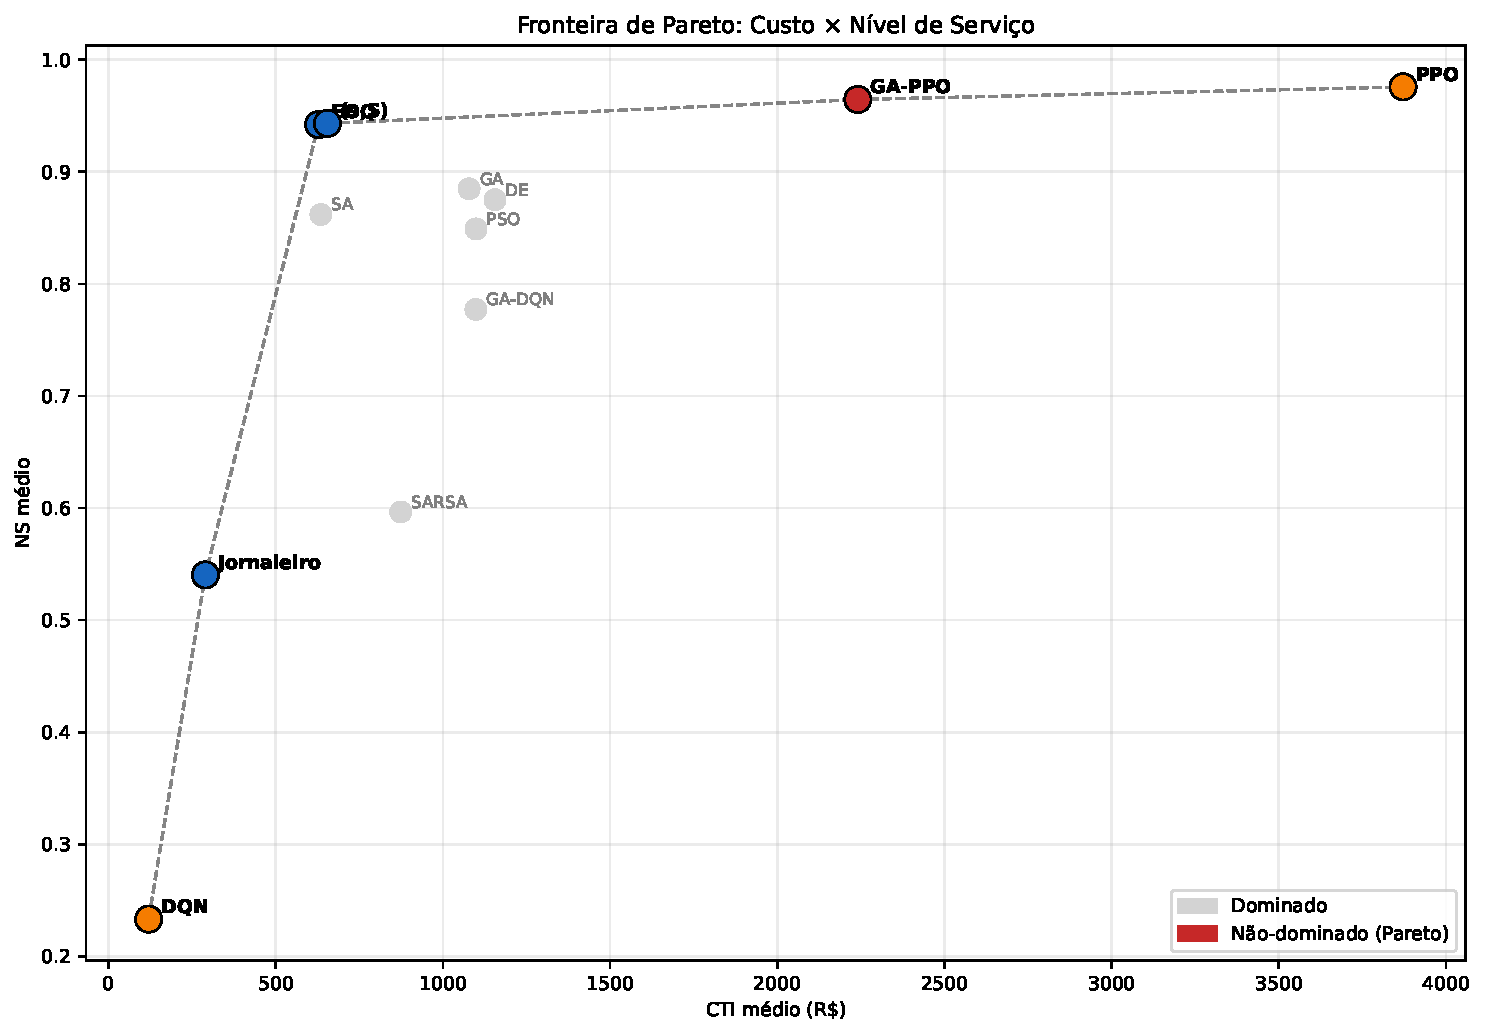
\includegraphics[width=0.62\linewidth,height=6.6cm,keepaspectratio]{figures/pareto_frontier.pdf}\\[0.4em]
  {\small Cada ponto é a média de uma política sobre as 145 séries da Bahia.}
  \note{
    Cada ponto representa a média de CTI e NS de uma política sobre as 145
    séries. O eixo horizontal é o custo, a ser minimizado; o eixo vertical é
    o nível de serviço, a ser maximizado. Nenhuma política ocupa
    simultaneamente o menor CTI e o maior NS -- não há dominância universal
    no recorte avaliado. Quem prioriza custo aponta para o Jornaleiro; quem
    prioriza serviço aponta para EOQ ou (s,S). Essa ausência de dominância
    universal é a evidência empírica direta que motiva a seleção contextual.
  }
\end{frame}
